\documentclass[a4paper,12pt]{report}
\usepackage[margin=1in]{geometry}
\usepackage{graphicx}
\usepackage[utf8]{vietnam}
\usepackage[english]{babel}
\usepackage{lmodern} 
\usepackage{parskip}
\usepackage{hyperref}

\renewcommand\thesection{\arabic{section}}
\renewcommand\thesubsection{\thesection.\arabic{subsection}}
\renewcommand\thesubsubsection{\thesubsection.\arabic{subsubsection}}

\begin{document}
\thispagestyle{empty}

\begin{center}
    \setlength{\fboxsep}{0pt}
    \setlength{\fboxrule}{0pt}
    \fbox{
        \begin{minipage}{\textwidth}
            \begin{minipage}{0.3\textwidth}
                
\includegraphics[width=\textwidth]{usth_logo.png}
            \end{minipage}
            \hfill
            \begin{minipage}{0.65\textwidth}
                \raggedright
                \textbf{\large University of Science and Technology of Hanoi}
            \end{minipage}
        \end{minipage}
    }
    \vspace{1cm}
    \\
    \textbf{\Large Distributed Systems} \\
    \textbf{\large Midterm Report} \\
    \vspace{1cm}
    \rule{\textwidth}{0.5pt}
    \vspace{0.5cm}
    \\
    \textbf{\large Distributed Database: Database Replication} \\
    \vspace{0.5cm}
    \rule{\textwidth}{0.5pt}
    \vspace{1cm}
    \\
    Quang Vo Hong [\href{mailto:quangvh.22bi13386@usth.edu.vn}{quangvh.22bi13386@usth.edu.vn}] \\
    Tam Nguyen Duc [\href{mailto:tamnd.22bi13400@usth.edu.vn}{tamnd.22bi13400@usth.edu.vn}] \\
    Quang Le Anh [\href{mailto:quangla.22bi13380@usth.edu.vn}{quangla.22bi13380@usth.edu.vn}] \\
    Nguyen Vu The Khoi [\href{mailto:nguyenvtk.22bi13344@usth.edu.vn}{nguyenvtk.22bi13344@usth.edu.vn}] \\
    Quan Hong Chu [\href{mailto:quanch.22bi13367@usth.edu.vn}{quanch.22bi13367@usth.edu.vn}] \\
    \vspace{2cm}
    Hanoi, December 2024
\end{center}

\newpage
\tableofcontents

\newpage
\section{\bfseries Introduction}
\fontsize{13}{16}\selectfont

\subsection{Context}
\hspace*{1em}A Distributed database is a database shared by multiple servers or computers instead of limited to one system. Inside a Distributed database system, each component contains its own database connected with other databases. A Distributed database has higher benefits than a centralized database system as it provides faster data processing between sites. It also ensures that the system can still execute if one or more sites fail to operate.

\hspace*{1em}One of the most important parts of a Distributed database is Replication. Replication is a method used for storing data. In the Replication approach, systems maintain copies of data stored in multiple sites instead of only one main copy in the main site. With Replication, data can be accessed at different sites in parallel. The system is also ensured to continue to operate even if a server fails as there are copies of the same data on different other servers. 

\hspace*{1em}Following the Replication method, MySQL Replication is a process that can automatically copy data from one MySQL server to other replica servers. The replica servers are proposed to be updated from the source’s data. 

\hspace*{1em}The efficient synergy between MySQL and the Replication method is widely used for numerous purposes:
\begin{itemize}
    \item Balancing Loads: Queries can be redirected to replica servers in order to reduce the load on the source server.
    \item System Availability: MySQL Replication can ensure the source system can still operate in case one or more servers fail to operate.
    \item Backup Solution: Replica servers can be used for backups without interaction with the main database.
    \item Disaster Recovery: A replica server can be quickly promoted to the primary server in the event of catastrophic failures.
\end{itemize}

\subsection{Objectives}
\hspace*{1em}Our main objective is building a MySQL Master-Slave Replication system. The system can copy and update data from a primary database (Master database) to one or more secondary databases (Slave databases). The Master database will receive all write operations including inserts, updates, deletions, etc… After the Master database is modified, a copy of it will be kept in a Slave database. The copy process will be executed automatically whenever the master database is altered.

\subsection{Outcomes}
\hspace*{1em}A MySQL Master-Slave Replication system can automatically copy the Master database to a Slave database every time the Master database is modified.

\section{\bfseries Methodology}
\fontsize{13}{16}\selectfont
\subsection{System Architecture}
Our system consists of 5 components: Master Database, Master Server, Message Bus, Slave Server and Slave Database. User will interact with the Master Database to perform write operations. The modifications will be forwarded to Message Bus and a Slave Database will be created for storing a copy of the Master Database.

\begin{figure}[h!]
    \centering
    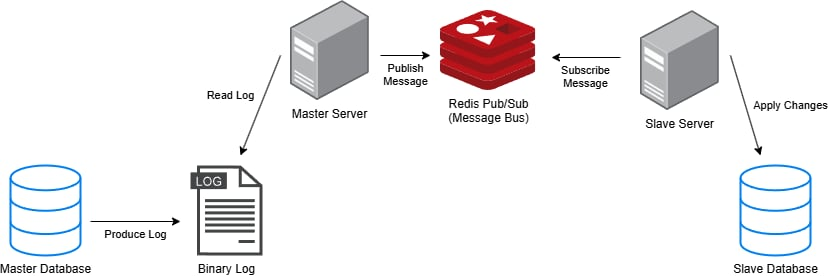
\includegraphics[width=\textwidth]{distribute_system_architecture.png}
    \caption{System Architecture}
    \label{fig:system_architecture}
\end{figure}

\subsection{Role Assignments}

Each component of the system plays an important role in the system:

\subsubsection{Master Database}
The Master Database is the system source database. It will handle all write operations and create a binary log whenever there is a modification to the database.

\subsubsection{Master Server}
The Master Server can access binary logs created by the Master Database. It will extract the modifications of the database from the binary logs. The Master Server publishes to a Redis Pub/Sub channel for sending modifications messages.

\subsubsection{Message Bus}
The Message Bus is used for connecting messages between the Master Server and the Slave Server. It act as a layer for multiple Slave Server interact with the Master Server at the same time. We use Redis Pub/Sub for creating channels for transmitting data between Servers.

\subsubsection{Slave Server}
The Slave Server subscribe to a Redis Pub/Sub channel for receiving modifications messages. It will then update and apply to the Slave Database to create a copy of the Master Database.

\subsubsection{Slave Database}
The Slave Database is a copy of the Master Database enabled with read operations. Each Slave Database contains a copy of the Master Database after each modification made to the source database.

\newpage
\end{document}
